\documentclass[12pt]{article}
\usepackage[czech]{babel}
\usepackage{epsf,epic,eepic,eepicemu, graphicx}
%\documentstyle[epsf,epic,eepic,eepicemu]{article}

\usepackage[T1]{fontenc}
\usepackage[utf8]{inputenc}
\usepackage{cmap}
\usepackage{mathpazo}

\begin{document}
%\oddsidemargin=-5mm \evensidemargin=-5mm \marginparwidth=.08in
%\marginparsep=.01in \marginparpush=5pt \topmargin=-15mm
%\headheight=12pt \headsep=25pt \footheight=12pt \footskip=30pt
%\textheight=25cm \textwidth=17cm \columnsep=2mm \columnseprule=1pt
%\parindent=15pt\parskip=2pt

\begin{center}
\bf České vysoké učení technické v Praze\\[2mm]
	Fakulta informačních technologií\\[2mm]
	Thákurova 9, 160 00, Praha 6\\[15mm]
	\textbf{Semestralní projekt MI-PAR 2011/2012:\\
    Paralelní algoritmus \\
    zobecněné Hanojské věže}\\[5mm]
       Jaroslav Hejral\\
       Jan Langer\\[2mm]
\today\\[12mm]
\end{center}

\section{Definice problému a popis sekvenčního algoritmu}
Algoritmus úlohy řeší problém sestavení postupu tahů k vyřešení zoběcněných Hanojských věží pro počet věží větší než 3. Hanojská věž o výšce k je věž k různých žetonů, které jsou uspořádány od nejmenšího k největšímu a rozdíly ve velikostech sousedních žetonů jsou vždy 1. Neuplná hanojská věž o výšce k je věž k různých žetonů, které jsou uspořádány od nejmenších k největším a rozdíly ve velikostech alespoň 1 dvojice sousedních žetonů je alespoň 2. Jeden tah je přesun disku z jedné tyče na jinou s tím, že cílová tyč je buď prázdná nebo je na jejím vrcholu disk s větším průměrem. Úkolem algoritmu je sestavit na cílové tyčce úplnou hanojskou věž s minimálním počtem tahů.

\subsection{Vstupní data}
\begin{itemize}
\item n = přirozené číslo představující celkový počet žetonů, n >= 16. Žeton i, i=1,..,n, má průměr i
\item s = přirozené číslo představující počet tyček, n/4 >=s > 3
\item r = číslo cílové tyčky, 1 <= r <= s
\item V[1,..,s] = množina neúplných hanoiských věží.
\end{itemize}

Argument V se zadává pomocí skóre jednotlivých věží. Skóre tyče je desítková reprezentace binárního kódu představujícího velikosti disků umístěných na konkrétní tyči. Vypočte se pomocí vzorce:
\begin{center}
$\displaystyle\sum\limits_{i=0}^n {2^{d(i)-1}}$
\end{center}
 kde n=počtu disků na tyči a d(i)=velikosti disku. Součet skóre všech tyčí musí být rovno $2^{n-1}$.

Příklad volání programu s parametry:
\texttt{./mi-par 5 4 4 1:30:0:0}

\begin{figure}[h]
\begin{center}
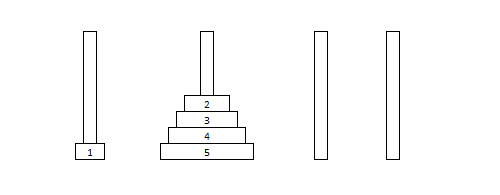
\includegraphics[width=140mm]{5-4-4.png}
\caption{Počáteční konfigurce pro zadání \texttt{./mi-par 5 4 4 1:30:0:0}}
\end{center}
\end{figure}



\subsection{Výstup algoritmu}
Výstupem algortmu je výpis počtu tahů a posloupnost tahů ve formátu disk, původní tyč -> cílová tyč.
Přiklad výstupu pro ukázkové zadání:

\begin{verbatim}
-------------
I have solution!
Number of moves: 12
2: 2 > 4;
3: 2 > 3;
2: 4 > 3;
1: 1 > 3;
4: 2 > 1;
5: 2 > 4;
1: 3 > 2;
4: 1 > 4;
2: 3 > 1;
3: 3 > 4;
2: 1 > 4;
1: 2 > 4;
\end{verbatim}
\subsection{Popis sekvenčního algoritmu}
Algoritmus je typu BB-DFS, tedy prohledávání do hloubky s návratem a mezí. Řešení algoritmu vždy existuje. 

V každém cyklu sekvenčního algoritmu je odebrán prvek na vrcholu zásobníku. Je zkontrolováno, zda-li jsme nedošli k řešení, pokud ano je řešení uloženo, sníží se horní mez a smyčka se spustí znovu. Pokud ne, zkontroluje se dosažení meze a zda-li existují možnosti přesunu disků do dalšího kroku. V případě je možné nějaké disky přesunout, vygenerují se  a vloží do zásobníku. Smyčka běží dokud není prázdný zásobník. Na konci běhu program vypíše nalezené řešení a počet tahů.

\subsubsection{Optimalizace ořezávání horní mezí}
Těsná horní mez řešení se vypočte podle vzorce $(2^{n/(s-2)-1})(2s-5)$. V případě že je nalezeno řešení je horní mez snížena na jeho velikost mínus jedna (hledáme o jedno menší řešení). Pokud zanoření ve stromu řešení překročí aktuálně platnou horní mez dojde k oříznutí této neperspektivní větve a provede se návrat. 

Ořezávání se nám ještě podařilo optimalizovat, a to tak, že návrat se provede už v případě, že aktuálně zbývající počet kroků do horní meze již nestačí pro přesunutí všech zbývajících disků na cílovou tyč. Touto optimalizací můžeme dosáhnout oříznutí neperspektivního postupu až o (horní mez-počet disků) dříve. Její významnost se zvyšuje s přibývajícím množstvím disků.

\section{Popis paralelního algoritmu a jeho implementace v MPI}
Algoritmus je typu \verb|G-PBB-DFS-D|. Oproti zádání jsme upravili způsob
šíření nejlepšího známého řešení, které jsme se rozhodli sdílet globálně. Vedla
nás k tomu především vidina značné uspory ve výpočtech. Procesor, který nalezne
řesení (které z podstaty úlohy vždy existuje) sdílí jeho délku s ostatními
procesory. To nám u nich umožní rychleji zaříznout částečná řešení, která již
nemají šanci na to býti lepšími.

\subsection{Pracovní smyčka}
Hlavní smyčka programu, která slouží pro řešení problému je prováděna dokud má
daný procesor něco na práci (v zásobníku disponuje nějakým částečným řešením,
které ještě neprozkoumal). Kromě standardního výpočtu řešení, který odpovídá
sekvenčnímu algoritmu obsahuje neblokovanou detekci příchodu zpráv. V této
části je kódu můžou přijít následující zprávy.

\begin{description}
  \item [TAG\_NEED\_MORE\_WORK] Některý procesor žádá práci. Pokud danému 
procesoru ještě zbývá nějaká práce v zásobníku, tak žadateli pošle práci ze 
dna zásobníku. Distribucí práce ze spodku zásobníku jsme dosáhli značného 
zrychlení kde máme jistotu, že předané částečné řešení má největší potenciál 
další řešitelnosti.
  \item [TAG\_SOLUTION\_NEW\_LIMIT] Tato zprávu rozesílá pouze hlavní
procesor(P0). Každý procesor, který ji přijme si upraví vlastní limit určující
novou horní mez pro hledání řešení. 
  \item [TAG\_FINALIZE] Tato zprávu rozesílá pouze předchůdce a nejedná
se o nic jiného než o peška. Při přijmu se provede logický součin peška s
vlastním indikátorem práce. Agresivní je v tomto přípádě 0, která reprezentuje
existenci práce. V rámci hlavní smyčky je krajně nepravděpodobné, že by procesor
dále poslal že nemá práci. Jediný případ, kdy by to mohlo nastat je, když by
procesor těsně před přijmutím peška odeslal poslední částečné řešení žadateli o
práci.
\end{description}
V neposlední řadě se v rámci pracovní smyčky kontroluje dosažení řešení. V
případě, že procesor najde řešení splňující kriteria pošle toto řešení hlavnímu
procesoru(P0). Posílá mu počet kroků vedoucí k řešení a řešení jako takové.
Hlavní procesor na to reaguje tak, že napřed porovná počet kroků s jeho
aktuálním limitem a pokud je dané řešení kratší, uloží si jej a pošle všem
procesorům zprávu \verb|TAG_SOLUTION_NEW_LIMIT| s novým limitem.

\subsection{Čekací smyčka}
Do čekací smyčky se procesor dostane v případě, že mu dojde práce. Postupně
neblokovaně žádá o práci a následně čeká na přijetí jedné z následujících zpráv.
\begin{description}
  \item [TAG\_SIZE\_OF\_NEW\_WORK] Jedná se o první ze dvou zpráv s novou prací.
Principielně procesor požádal o práci a také ji dostal. Získanou práci si vloží
do zásobníku, změní svůj stav na to, že má práci a opustí smyčku hledání práce.
  \item [TAG\_FINALIZE] Jedná o peška. Pokud mi je poslán v tuto chvíli vím, že
nejsem jeho autorem, a proto ho pouze logicky přenásobím se svým stavem a sice
nemám práci (logická 1). Opět platí agresivita nuly (je práce).  
  \item [TAG\_NO\_MORE\_WORK] Tuto zprávu očekávám pouze od toho procesoru,
kterého jsem žádal o práci. Indikuje danému procesoru fakt, že ani dotazovaný
nemá nic na práci a proto se musí poohlédnout jinde.
  \item [TAG\_NEED\_MORE\_WORK] Někdo od daného procesoru žádá práci. Bohužel
ji nemá a proto rovnou odpoví zprávou \verb|TAG_NO_MORE_WORK|.
   \item [TAG\_TERMINATE] Někdo rozhodl, že je na čase ukončit výpočet. Po
přijmu napřed daný procesor přepošle asynchronně stejnou zprávu svému
následovníkovi. Hlavní procesor (P0) vypíše na stardandní výstup
řešení a ukončí se. Jiný než hlavní procesor se pouze ukončí.
\end{description}
V případě, že opouští procesor část čekací smyčky ve které si řešil hledání
prace a tento proces byl úspěšný, vrátí se do pracovní smyčky. V případě
neúspěchu začne šířit peška. Blokovaně čeká na jeho návrat od předchudce. Pokud
se pešek vrátí s tím, že někde ještě práce je, vrátí se do části vyhledávání
práce. Pokud se však pešek vratí s tím, že už nikde není práce, začne
procesor šířit zprávu  \verb|TAG_TERMINATE| a ukončí se.
\subsection{Hledání dárce}
Pro hledání dárce jsme se rozhodli použít pseudo-náhodný přistup. Procesor,
kterému dojde práce si náhodně určí první procesor, kterého požádá o práci.
Pokud od něj práci nedostane tak požádá jeho následovníka. Toto se opakuje
dokud nevyčerpá všechny možnosti.

\subsection{Ukončení výpočtu}
Pro ukončení výpočtu používáme stardandní kolečko s peškem. Peška začne posílat
procesor, který nemá prací i poté, co o ní požádal postupně všechny ostatní procesy. 
Každý kdo peška přijme ho přebarví podle toho, jestli práci má nebo ne.
Případ, kdy přijde pešek v momentě kdy procesor poslal práci do části, kde již pešek
byl, máme ošetřen tím, že v tu chvíli se daný procesor tváří jako by sám práci
měl, i když to nemusí být nezbytně pravda. Když se pešek vrátí k procesoru který ho vyslal, 
a je ve stavu \uv{není práce} (logická 1), informuje svého následníka o ukončení výpočtu. 
Každý procesor, který zprávu o ukončení obdrží ji přepošle svému následovníkovi a ukončí se.
Jedinou vyjímkou v pravidlu je hlavní procesor (P0), který před svým ukončením
vypíše na výstup nalezené řešení.

\subsection{Sémantika příkazu}
Oproti sekvenčnímu řešení nedoznala sémantika příkazu žádných změn. 
\begin{verbatim}
  ./mi-par 5 4 4 1:30:0:0                 
\end{verbatim}

\section{Naměřené výsledky a vyhodnocení}

Výslednou aplikaci jsme otestovali na výpočetním stroji STAR pro tři různě velké instance problému. Každé zadání bylo změřeno pro běh na 1, 2, 4, 8, 16 a 24 procesorech a pro komunikační sítě InfiniBand a Ethernet. Měření na svazku STAR probíhalo vždy na uzlech s 12 jádry (parametr \textit{12c} při spuštění).

\begin{itemize}
\item Zadání č. 1: \texttt{16 6 6 72:32:3:0:20:65408}
\item Zadání č. 2: \texttt{16 7 7 72:32:3:0:20:0:65408}
\item Zadání č. 3: \texttt{16 9 9 72:32:3:128:20:0:0:0:65280}



\end{itemize}

\begin{figure}[h]
\begin{center}
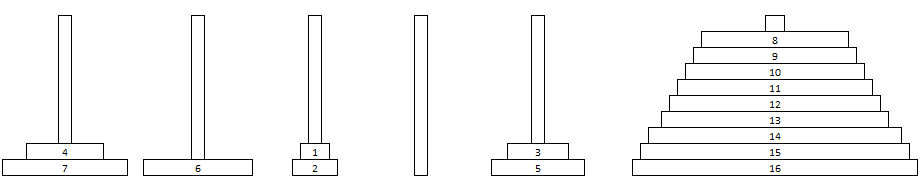
\includegraphics[width=140mm]{16-6-6.png}
\caption{Zadání č. 1: 16 disků, 6 tyčí, cílová tyč č. 6}
\end{center}
\end{figure}

\begin{figure}[h]
\begin{center}
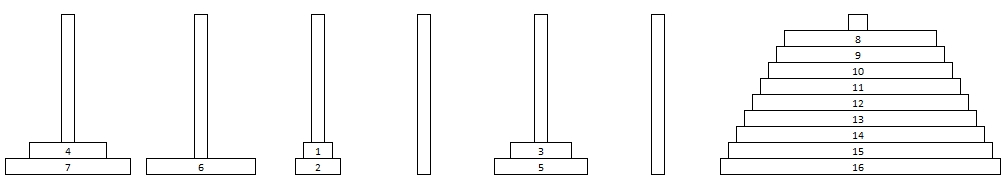
\includegraphics[width=140mm]{16-7-7.png}
\caption{Zadání č. 2: 16 disků, 7 tyčí, cílová tyč č. 7}
\end{center}
\end{figure}

\begin{figure}[h]
\begin{center}
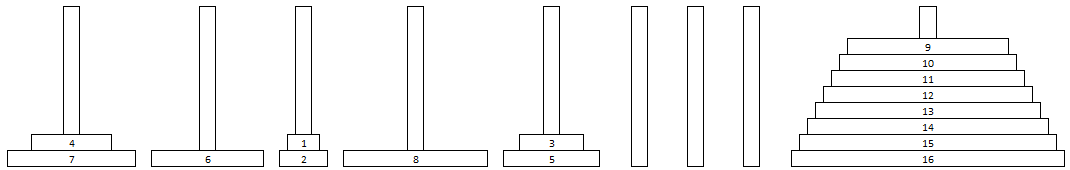
\includegraphics[width=140mm]{16-9-9.png}
\caption{Zadání č. 3: 16 disků, 9 tyčí, cílová tyč č. 9}
\end{center}
\end{figure}


\subsection{Naměřené výsledky pro síť InfiniBand 10Gbps}
\begin{center}
\begin{tabular}{|c|c|c|c|}
\hline 
 & \multicolumn{3}{c|}{čas [s] (zaokrouhleno na 1 desetiné místo)} \\ 
\hline 
počet procesů & Zadání č.1 & Zadání č.2 & Zadání č.3 \\ 
\hline 
\hline 
1 & 2387,5 & 379,2 & 1251,2 \\ 
\hline 
2 & 1095,8 & 202,9 & 793,0 \\ 
\hline 
4 & 289,1 & 36,1 & 415,5 \\ 
\hline 
8 & 177,8 & 35,5 & 228,1 \\ 
\hline 
16 & 176,6 & 35,7 & 224,2 \\ 
\hline 
24 & 175,4 & 34,9 & 220,9 \\ 
\hline 
\end{tabular} 
\end{center}


\begin{figure}[h]
\begin{center}
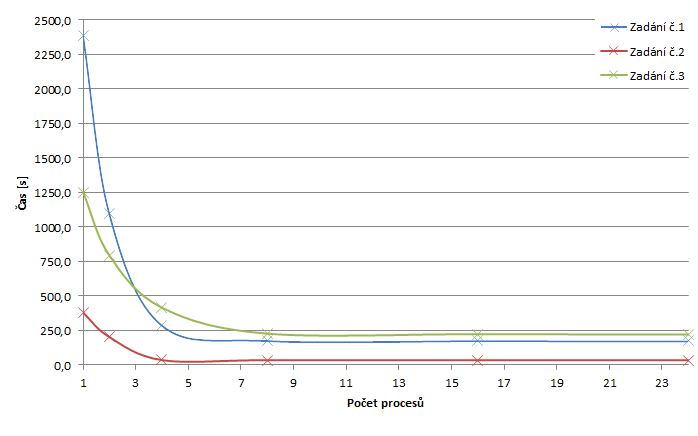
\includegraphics[width=100mm]{cpu_time_inifiniband.png}
\caption{Rychlost výpočtu v závislosti na počtu procesů (InfiniBand)}
\label{fig:ct_inifini}
\end{center}
\end{figure}

\begin{figure}[h]
\begin{center}
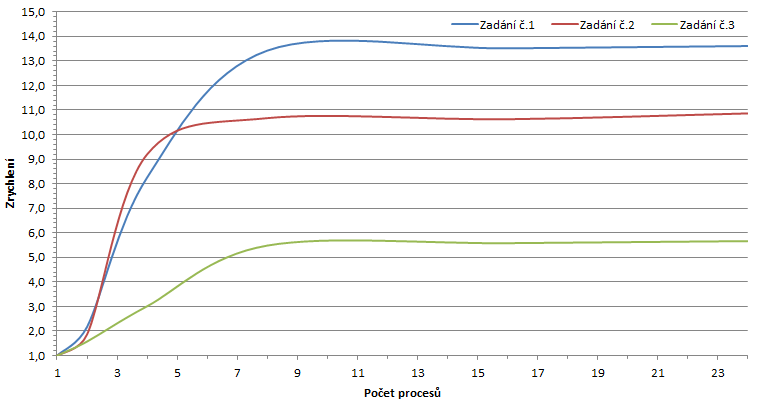
\includegraphics[width=100mm]{speedup_infini.png}
\caption{Zrychlení výpočtu v závisloti na počtu procesů (InfiniBand)}
\label{fig:speedup_inifini}
\end{center}
\end{figure}

\subsection{Naměřené výsledky pro síť Ethernet 1Gbps}

\begin{center}
\begin{tabular}{|c|c|c|c|}
\hline 
 & \multicolumn{3}{c|}{čas [s] (zaokrouhleno na 1 desetiné místo)} \\ 
\hline 
počet procesů & Zadání č.1 & Zadání č.2 & Zadání č.3 \\ 
\hline 
\hline 
1 & 2387,5 & 379,2 & 1251,2 \\ 
\hline 
2 & 1151,3 & 205,5 & 798,4 \\ 
\hline 
4 & 294,2 & 41,2 & 435,5 \\ 
\hline 
8 & 181,4 & 37,0 & 235,5 \\ 
\hline 
16 & 181,9 & 36,1 & 227,1 \\ 
\hline 
24 & 181,7 & 35,4 & 221,1 \\ 
\hline 
\end{tabular} 
\end{center}

\begin{figure}[h]
\begin{center}
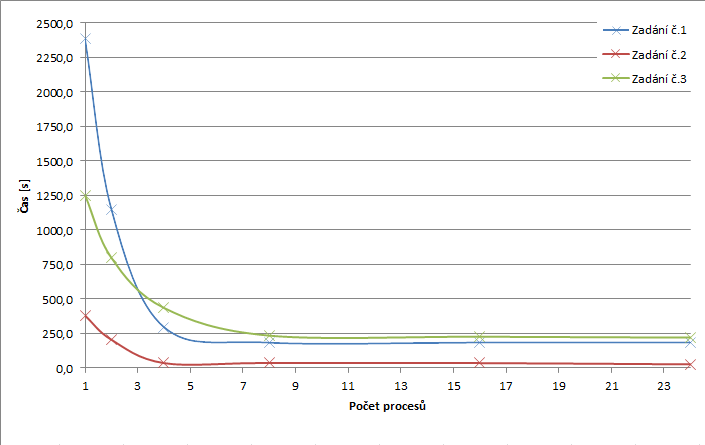
\includegraphics[width=100mm]{cpu_time_ethernet.png}
\caption{Rychlost výpočtu v závislosti na počtu procesů (Ethernet)}
\label{fig:ct_inifini}
\end{center}
\end{figure}


\subsection{Porovnání měření na Infinibandu a Ethernetu}
Z porovnání hodnot naměřených na síti Infiniband a Ethernet je vidět, že rozdíli dosahují maximálně desítek sekund pro větší instance na menším počtu procesorů. Částečný vliv na hodnoty má samozřejmě také momentální zatížení svazku STAR a jeho komunikačních sítí v době měření. V procentuálních hodnotách má nějvětší rozdíl hodnotu 5\% pro zadání č.1 na 2 jádrech, pro menší instance a také větší počet procesorů jsou ale rozdíly menší a tak můžeme říci, že rozdílná rychlost přenosu mezi uzly nemá na celkovou dobu výpočtu zásadní vliv.

\section{Závěr}

Úspěšně se nám podařilo implementovat sekvenční i paralelní algoritmu pro řešení zadaného problému.
Provedli jsme měření času potřebného pro výpočet  úloh netriviální složitosti sekvenčně a paralelně na 1-24 jádrech procesoru.
Výsledky měření ukazují, že algoritmus vykazuje na více procesorech superlineární zrychlení, a to především proto, že současným 
výpočtem ve více větvích stromu dokážeme dříve nalézt \uv{neideální} řešení a tedy snižovat horní mez, která je globálně sdílena.

Semestrální práce pro nás byla velkým přínosem, hlavně co se týká seznámení s MPI a komunikací v paralelním prostředí. 

\end{document}
